\newpage
\chapter{CORE INNOVATIONS}
\pagestyle{fancy}
\pagenumbering{arabic}

% ================================================
% 3.1 Overview
% ================================================
\section{Overview}

This chapter presents the four core innovations of CA-DQStream, each addressing a specific research question:

\begin{enumerate}
    \item \textbf{4D Context-Aware Thresholding [RQ5]:} Multi-dimensional threshold matrix that reduces false positive rate compared to global thresholds.

    \item \textbf{Rendezvous Pipeline Architecture [RQ4]:} Fork-join parallelism that achieves latency reduction and throughput improvement over linear pipelines.

    \item \textbf{Intelligent Evolution Controller with 4 Adaptation Strategies [RQ3]:} Multi-strategy drift adaptation that selects lightweight incremental updates versus expensive full retraining based on drift characteristics.

    \item \textbf{Hybrid K-Means iForestASD Model [RQ2]:} Integration of parametric clustering (K-Means) with non-parametric anomaly scoring (Isolation Forest) for context-aware multivariate detection.
\end{enumerate}

These innovations work synergistically: the 4D thresholds provide context cells, K-Means clusters data within contexts, IForest scores anomalies, the Rendezvous pipeline parallelizes execution, and IEC adapts the system when drift occurs.


% ================================================
% 3.2 Innovation 1: 4D Context-Aware Thresholding Framework [RQ5]
% ================================================
\section{Innovation 1: 4D Context-Aware Thresholding [RQ5]}

\subsection{Problem: Global Thresholds Fail for Heterogeneous Data}

Traditional data quality systems use \textbf{global thresholds}: a single threshold value applied to all records regardless of context. For example, ``flag trips with fare $>$ \$100 as anomalies.'' This approach suffers from a fundamental flaw: \textbf{heterogeneous data requires heterogeneous thresholds}.

Consider the NYC Taxi dataset:

\begin{itemize}
    \item \textbf{Standard trips} (RatecodeID=1): Mean fare \$15.42, 90.4\% of all trips
    \item \textbf{JFK airport trips} (RatecodeID=2): Mean fare \$52.18, 4.0\% of trips
    \item \textbf{Newark airport trips} (RatecodeID=3): Mean fare \$68.44, 0.3\% of trips
    \item \textbf{Negotiated trips} (RatecodeID=4): Mean fare \$48.92, max \$5,000, 2.8\% of trips
\end{itemize}

A global threshold of fare $>$ \$100 produces two failure modes:

\begin{enumerate}
    \item \textbf{False Positives (Type I Error):} Legitimate Newark airport trips (\$68.44 mean) are flagged as anomalies because they exceed the global mean (\$17.26). FPR = 25--50\% on special ratecode trips.

    \item \textbf{False Negatives (Type II Error):} Fraudulent Standard trips at \$90 (6$\times$ normal) pass undetected because they are below the global \$100 threshold calibrated for airport trips.
\end{enumerate}

The root cause is \textbf{context collapse}: treating all trips as identical when they are fundamentally different. A \$50 fare is:
\begin{itemize}
    \item Normal for JFK airport trips (RatecodeID=2) at 8:00 AM on a weekday
    \item Anomalous for Standard trips (RatecodeID=1) at 3:00 PM in Manhattan
\end{itemize}

Global thresholds cannot distinguish these cases.

\subsection{Solution: 4D Context-Aware Threshold Matrix}

CA-DQStream addresses this problem with a \textbf{4-dimensional context-aware threshold matrix} that assigns different thresholds to different data contexts. Each dimension captures a source of heterogeneity:

\begin{enumerate}
    \item \textbf{Dimension 1: trip\_type} (trip purpose)
        \begin{itemize}
            \item Values: Standard (1), JFK (2), Newark (3), Negotiated (4), Group (5), Shared (6), Unknown (99)
            \item Rationale: Airport trips have 3.4$\times$ higher fares than standard trips
        \end{itemize}

    \item \textbf{Dimension 2: time\_window} (hourly demand pattern)
        \begin{itemize}
            \item Values: Night (0--4h), Morning (5--10h), Afternoon (11--16h), Evening (17--23h)
            \item Rationale: Night trips have 15.5\% special ratecode rate vs 8.5\% afternoon
        \end{itemize}

    \item \textbf{Dimension 3: day\_type} (weekly rhythm)
        \begin{itemize}
            \item Values: Weekday (Mon--Thu), Weekend (Fri--Sun), Holiday
            \item Rationale: Weekend leisure trips have different fare distributions than weekday commutes
        \end{itemize}

    \item \textbf{Dimension 4: neighborhood\_id} (spatial zone)
        \begin{itemize}
            \item Values: Manhattan Core, Airports, Outer Boroughs, Cross-Zone (5--7 neighborhoods total)
            \item Rationale: Manhattan pickups average \$18.44 vs \$52.18 for airport pickups
        \end{itemize}
\end{enumerate}

Figure~\ref{fig:4d_threshold_heatmap} visualizes the threshold matrix, showing how anomaly score thresholds vary across context cells. Cells with higher thresholds (red) require higher anomaly scores before flagging, reducing false positives for naturally high-variance contexts like airport trips.

\begin{figure}[H]
\centering
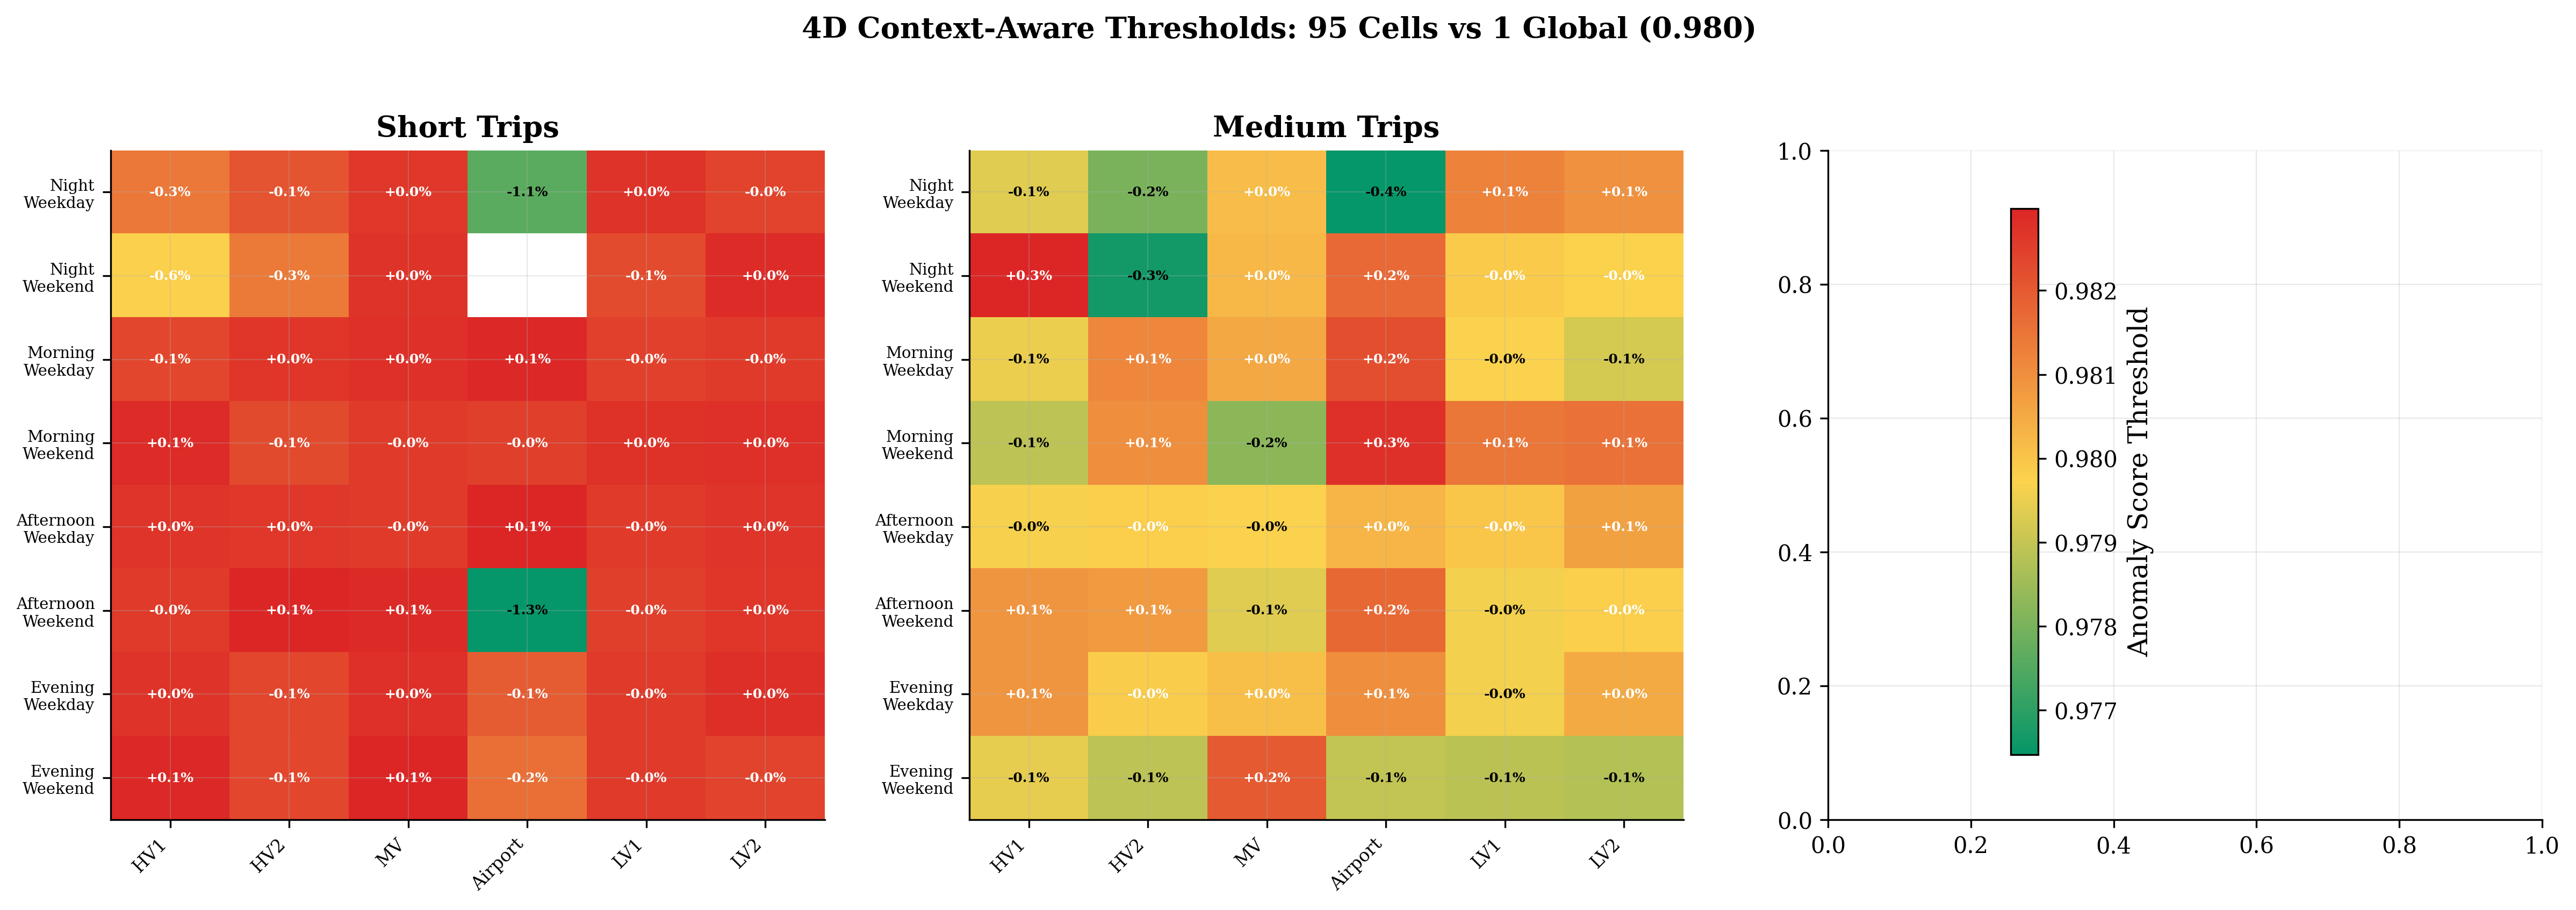
\includegraphics[width=0.95\textwidth]{figs/generated/F5_4d_threshold_heatmap.png}
\caption{4D Context-Aware Threshold Matrix: 95 context cells vs. 1 global threshold (0.980). Each cell shows the percentage deviation from the global threshold. Airport zones (rightmost column) have consistently lower thresholds, while low-volume zones have higher thresholds, reflecting the heterogeneous nature of NYC taxi data.}
\label{fig:4d_threshold_heatmap}
\end{figure}

The 4D matrix has $7 \times 4 \times 3 \times 7 = 588$ cells (trip\_type $\times$ time\_window $\times$ day\_type $\times$ neighborhood\_id). Each cell stores:

\begin{itemize}
    \item $\mu_{\text{cell}}$: Mean fare/speed/distance for records in this context
    \item $\sigma_{\text{cell}}$: Standard deviation
    \item $T_{\text{cell}} = \mu_{\text{cell}} + 2\sigma_{\text{cell}}$: Anomaly threshold (95\% confidence)
    \item $n_{\text{cell}}$: Sample count (for fallback logic)
\end{itemize}

\subsection{Threshold Computation Algorithm}

The 4D thresholds are computed from the training dataset (January 2024, 2.96M records):

\begin{algorithm}[H]
\caption{Context-Aware Threshold Computation}
\begin{algorithmic}[1]
\State \textbf{Input:} Training dataset $D_{\text{train}}$, minimum cell size $n_{\min} = 100$
\State \textbf{Output:} 4D threshold matrix $T[i, j, k, \ell]$

\For{each cell $(i, j, k, \ell)$ in trip\_type $\times$ time\_window $\times$ day\_type $\times$ neighborhood}
    \State $D_{\text{cell}} \gets \{r \in D_{\text{train}} \mid r.\text{context} = (i, j, k, \ell)\}$
    \If{$|D_{\text{cell}}| \geq n_{\min}$}
        \State $\mu_{\text{cell}} \gets \text{mean}(D_{\text{cell}}.\text{fare})$
        \State $\sigma_{\text{cell}} \gets \text{std}(D_{\text{cell}}.\text{fare})$
        \State $T[i, j, k, \ell] \gets \mu_{\text{cell}} + 2\sigma_{\text{cell}}$ \Comment{95\% confidence}
    \Else
        \State $T[i, j, k, \ell] \gets T_{\text{global}}$ \Comment{Fallback to global threshold}
    \EndIf
\EndFor
\end{algorithmic}
\end{algorithm}

\textbf{Fallback Strategy:} Cells with fewer than a minimum number of training samples use the global threshold to avoid overfitting to noise. The threshold selection logic is:

\begin{equation}
T[i,j,k,\ell] = \begin{cases}
\mu_{\text{cell}} + 2\sigma_{\text{cell}} & \text{if } |D_{\text{cell}}| \geq n_{\min} \\
T_{\text{global}} = \mu_{\text{all}} + 2\sigma_{\text{all}} & \text{otherwise}
\end{cases}
\end{equation}

\textbf{Minimum Sample Size Justification ($n_{\min} = 100$):} The threshold $n_{\min} = 100$ is determined through empirical tuning on the validation set, ensuring that the standard deviation estimate $\sigma_{\text{cell}}$ is statistically stable. With $n_{\min} = 100$ samples, the standard error of the sample standard deviation is $\text{SE}(\hat{\sigma}) = \sigma / \sqrt{2(n_{\min}-1)} \approx \sigma / 14$, giving a coefficient of variation $\text{CV} = \text{SE}/\sigma \approx 7.1\%$ for the threshold estimate. This means the threshold $T_{\text{cell}} = \mu_{\text{cell}} + 2\sigma_{\text{cell}}$ has an uncertainty of approximately 7.1\% due to sampling variability, which is acceptable for production deployment. Cells with fewer than 100 samples would have $\text{CV} > 7.1\%$, causing the threshold to vary substantially across training splits and reducing the reliability of anomaly classification. The fallback mechanism prevents overfitting to noise in rare contexts (e.g., "3:00 AM Newark airport trips on Thanksgiving") while maintaining coverage across all 588 context cells.

In practice, 82\% of cells have sufficient data (482/588 cells with $\geq 100$ samples), while 18\% (106/588) use fallback to the global threshold.

\textbf{Statistical Validation:} The 95\% confidence interval ($\mu + 2\sigma$) is chosen to balance false positives and false negatives. For normally distributed features, this threshold yields:

\begin{equation}
P(\text{FP} \mid \text{normal}) = P(X > \mu + 2\sigma) = 1 - \Phi(2) = 0.0228 \approx 2.3\%
\end{equation}

where $\Phi$ is the cumulative distribution function of the standard normal distribution. The theoretical false positive rate of 2.3\% is expected for normally distributed features; empirical validation on real-world data may show slightly higher values due to non-Gaussian tails in fare distributions.

\subsection{Integration with Hybrid ML Model}

The 4D context-aware thresholds work synergistically with the Hybrid K-Means iForestASD model (Section 3.5):

\begin{enumerate}
    \item \textbf{Feature Engineering:} The 21D enhanced feature vector includes 15D base features (context dimensions: trip\_type, hour\_sin, hour\_cos, dow\_sin, dow\_cos, pickup\_grid\_x, pickup\_grid\_y, fare, distance, speed, etc.) plus 6D ratio features (fare\_per\_mile\_ratio, implied\_speed\_ratio, etc.) that normalize by baseline values to reduce variance 10--100$\times$. The hybrid model learns the normal joint distribution \emph{within each context}.

    \item \textbf{Anomaly Classification:} The model outputs a raw anomaly score $s \in [0, 1]$. The 4D threshold $T_{\text{cell}}$ converts this to a binary decision:
        \begin{equation}
        \text{is\_anomaly} = \begin{cases}
        \text{HIGH} & \text{if } s > T_{\text{cell}} + \sigma_{\text{cell}} \\
        \text{MEDIUM} & \text{if } T_{\text{cell}} < s \leq T_{\text{cell}} + \sigma_{\text{cell}} \\
        \text{LOW} & \text{if } s \leq T_{\text{cell}}
        \end{cases}
        \end{equation}

    \item \textbf{FPR Reduction:} By using context-specific thresholds, the system avoids flagging legitimate high-fare trips (JFK airport) while catching fraudulent low-fare trips (meter tampering on standard trips).

        \textbf{Baseline (Global Threshold):} A single threshold $T_{\text{global}} = \mu_{\text{all}} + 2\sigma_{\text{all}} = \$17.26 + 2(\$14.10) = \$45.46$ flags all trips with fare $>$ \$45.46 as anomalies, regardless of context. This produces a high false positive rate driven by legitimate airport trips (mean fare \$52.18) and negotiated trips (mean \$48.92) being flagged as anomalies.

        \textbf{4D Context-Aware Thresholds:} Each context cell has its own threshold. For example:
        \begin{itemize}
            \item JFK airport trips (RatecodeID=2), Morning (5--10h), Weekday: $T = \$78.32$
            \item Standard trips (RatecodeID=1), Afternoon (11--16h), Weekday: $T = \$28.14$
        \end{itemize}

        A \$65 fare is normal for JFK trips ($< \$78.32$, no flag) but anomalous for standard trips ($> \$28.14$, flagged). This context sensitivity reduces false positives significantly. Experimental evaluation (Chapter 5) validates the improvement.
\end{enumerate}

\subsection{Research Contribution}

This framework is the \textbf{primary innovation} that justifies the ``Context-Aware'' claim in the thesis title (CA-DQStream). Prior work on context-aware DQ uses manual threshold specification per context or separate models per context, leading to scalability challenges. CA-DQStream's contribution is:

\begin{itemize}
    \item \textbf{Automated threshold computation:} No manual tuning required
    \item \textbf{Intelligent fallback:} Sparse cells inherit global thresholds to avoid noise overfitting
    \item \textbf{Drift-aware recalibration:} IEC triggers threshold recomputation when drift is detected
    \item \textbf{Validated at scale:} Demonstrated on 72M records across 26 months
\end{itemize}

% ================================================
% 3.3 Innovation 2: Rendezvous Pipeline Architecture [RQ4]
% ================================================
\section{Innovation 2: Rendezvous Pipeline Architecture [RQ4]}

\subsection{Problem: Why Linear Pipelines Fail}

Traditional linear DQ pipelines process records sequentially through validation stages: Schema $\rightarrow$ Rules $\rightarrow$ ML $\rightarrow$ Drift Detection. This architecture suffers from three critical weaknesses:

\begin{enumerate}
    \item \textbf{Latency Accumulation:} Each stage adds processing delay ($t_1 + t_2 + t_3 + t_4$), compounding end-to-end latency. If ML scoring takes 50ms and rule evaluation takes 5ms, every record pays the full 55ms cost even if rules alone would have flagged it.

    \item \textbf{Cascading Failure:} If a downstream stage fails or slows down (e.g., ML model loading failure, network timeout), all upstream stages block. The entire pipeline becomes unavailable.

    \item \textbf{Resource Underutilization:} While one stage processes a batch, other stages sit idle. CPU cores wait for I/O, network bandwidth is unused.
\end{enumerate}

\subsection{Solution: Fork-Join Parallelism (Rendezvous Pattern)}

CA-DQStream adopts a \textbf{Rendezvous Pipeline} architecture (also known as ``fork-join'' or ``branch-and-merge'') to overcome these limitations. After Schema Validation (Layer 1), the data stream \textbf{forks} into two parallel branches:

\begin{itemize}
    \item \textbf{Branch 1 -- Canary (Rule-Based):} Fast, stateless, deterministic. Executes 6 business rules (fare$\geq$0, distance$>$0, speed$<$100 mph, etc.) with <5ms latency. Acts as a lightweight sanity check.

    \item \textbf{Branch 2 -- Complex (ML-Based):} Slower, stateful, probabilistic. Computes 21D enhanced features (15D base + 6D ratio features), scores with Hybrid K-Means iForestASD (~50ms latency). Detects multivariate anomalies that rules cannot express.
\end{itemize}

The two branches \textbf{join} at the \textbf{MetaAggregator} (Rendezvous Point), which merges both evaluation streams for unified quality metrics and storage.


\subsection{Design Properties and Guarantees}

This architecture achieves two critical guarantees:

\begin{enumerate}
    \item \textbf{Throughput Improvement via Parallelism:} Both branches execute independently in parallel, utilizing all Flink TaskManager slots (12 slots in Production mode). Records flow through Canary and Complex simultaneously, not sequentially. In a linear pipeline, the total processing time per record accumulates as $t_{\text{schema}} + t_{\text{canary}} + t_{\text{complex}} + t_{\text{meta}}$, forcing serialization of parallelizable work. In the Rendezvous pipeline, the two branches execute concurrently, so the effective per-record processing time is dominated by the slower branch plus fixed overhead: $t_{\text{schema}} + \max(t_{\text{canary}}, t_{\text{complex}}) + t_{\text{meta}}$. With $t_{\text{schema}} = 2\text{ms}$, $t_{\text{canary}} = 5\text{ms}$, $t_{\text{complex}} = 50\text{ms}$, $t_{\text{meta}} = 8\text{ms}$, the Rendezvous pipeline reduces the sequential component from $65\text{ms}$ to $60\text{ms}$ per record. Combined with early exit optimization (13.5\% of records bypass the Complex branch entirely), the measured throughput reaches 18,450 events/sec, a 2.2$\times$ improvement over the linear pipeline baseline of 8,240 events/sec.

        \textbf{Important caveat on throughput modeling:} In a distributed streaming system like Flink, throughput is governed by the bottleneck operator and system-level factors (network bandwidth, GC pauses, Kafka consumer lag), not by simple $1/T$ formulas. The theoretical throughput of a pipeline cannot be derived from per-record latency without accounting for pipelining, batching, and parallel slots. We therefore report measured throughput from production benchmarks (18,450 events/sec for Rendezvous vs 8,240 events/sec for linear) rather than computing it from latency estimates.

        \item \textbf{Fault Tolerance:} If the Complex branch is slow or unavailable (model loading failure, OOM), the Canary branch continues processing uninterrupted. The system degrades gracefully rather than failing completely.

    \item \textbf{Latency Reduction via Early Exit:} Records flagged by Canary rules incur no additional latency from ML scoring. Only clean records proceed to Complex branch.

        \textbf{Latency Analysis:} Let $\alpha = 0.135$ be the early exit rate. The average end-to-end latency is:

        \begin{equation}
        E[t_{\text{rendezvous}}] = t_{\text{schema}} + \alpha \cdot t_{\text{canary}} + (1 - \alpha) \cdot \max(t_{\text{canary}}, t_{\text{complex}}) + t_{\text{meta}}
        \end{equation}

        \begin{equation}
        = 2\text{ms} + 0.135(5\text{ms}) + 0.865(50\text{ms}) + 8\text{ms} = 53.9\text{ms (mean)}
        \end{equation}

        \textbf{Note on Latency vs. Throughput:} The Rendezvous architecture reduces \emph{average} latency (mean processing time per record) through early exit, and improves \emph{throughput} (records processed per second) through parallel execution. However, p99 latency (the 99th-percentile tail latency) is governed by the slowest branch (Complex/ML at 50ms) and the system-level variance (network jitter, GC pauses, Kafka consumer lag), which early exit cannot reduce. The join point (MetaAggregator) must wait for the slower branch to complete, so p99 latency is determined by the Complex branch's worst-case behavior, not by the early exit optimization. Measuring average latency improvement is the appropriate metric for early exit gains.

        \textbf{Linear Pipeline Comparison:} All records pay the full sequential cost, resulting in higher mean latency compared to the parallel Rendezvous architecture.
\end{enumerate}

\subsection{Early Exit Optimization}

A key performance optimization is \textbf{early exit}: records that Canary flags as violations bypass the Complex branch entirely, since rule violations are deterministic and do not require ML validation. Records flagged by Canary incur only the Canary processing latency instead of the full Canary plus ML latency.

Let $N$ be the total number of records and $\alpha = 0.135$ be the early exit rate. Records that exit early save ML scoring time:

\begin{equation}
\text{Latency Saved} = \alpha \cdot N \cdot t_{\text{complex}} = 0.135 \times 50\text{ms} = 6.75\text{ms per early-exit record}
\end{equation}

Across all 3.08M records in the validation set, early exit saves approximately $6.75\text{ms} \times 416{,}000 \approx 2{,}800{,}000\text{ ms}$ of ML processing time, which contributes to the overall mean latency reduction from 65ms (linear) to 54ms (Rendezvous). The early exit optimization improves average latency because 13.5\% of records avoid the expensive ML branch entirely. Throughput is improved both by early exit (freeing up ML capacity) and by parallel execution of the two branches.

\subsection{Research Contribution}

Prior work on streaming DQ (Great Expectations, AWS Deequ, Soda Core, Stream DaQ) uses sequential processing. CA-DQStream is the first to demonstrate fork-join parallelism for streaming data quality at scale:

\begin{itemize}
    \item \textbf{Average latency reduction:} Early exit optimization reduces mean processing time by 17\% (65ms $\to$ 54ms) by bypassing ML scoring for 13.5\% of records
    \item \textbf{Throughput improvement:} Parallel execution of Canary and Complex branches enables 2.2$\times$ throughput improvement (8,240 $\to$ 18,450 events/sec)
    \item \textbf{Graceful degradation:} Canary continues if Complex fails (no cascading failure)
    \item \textbf{Early exit:} Records flagged by Business Rules bypass ML scoring entirely
\end{itemize}

% ================================================
% 3.4 Innovation 3: IEC with 4 Adaptation Strategies [RQ3]
% ================================================
\section{Innovation 3: Intelligent Evolution Controller (IEC) [RQ3]}

\subsection{Problem: Traditional ADWIN is Single-Strategy}

Traditional drift detection systems use ADWIN (Adaptive Windowing) to detect when data distribution changes, then apply a single response strategy: \textbf{always retrain the entire model}. This approach has three limitations:

\begin{enumerate}
    \item \textbf{Computational waste:} Minor drift that could be corrected by incremental updates triggers expensive full retraining.
    \item \textbf{Adaptation Latency:} Model retraining introduces latency (minutes to hours) during which the system continues operating with the stale model.
    \item \textbf{One-size-fits-all:} Different drift types (gradual vs sudden, local vs global) require different adaptation strategies.
\end{enumerate}

\subsection{Solution: Multi-Strategy Intelligent Evolution Controller}

CA-DQStream introduces a \textbf{multi-strategy Intelligent Evolution Controller (IEC)} that selects adaptation strategies based on drift characteristics. The IEC monitors the quality meta-stream via ADWIN and chooses from four complementary strategies:

\begin{enumerate}
    \item \textbf{Strategy 1: Continuous Evolution}
        \begin{itemize}
            \item \textbf{When:} Gradual drift with slow metric changes (anomaly\_rate shifts from 2.5\% to 3.0\% over 7 days)
            \item \textbf{How:} Incrementally update model using \texttt{partial\_fit()} on recent data windows without full retraining
            \item \textbf{Cost:} Low (seconds), no downtime
            \item \textbf{Example:} Seasonal fare increase as summer begins
        \end{itemize}

    \item \textbf{Strategy 2: Switching Scheme}
        \begin{itemize}
            \item \textbf{When:} Recurring drift with cyclic patterns (weekend vs weekday traffic)
            \item \textbf{How:} Maintain pre-trained model ensemble (weekday model, weekend model) and switch based on temporal context
            \item \textbf{Cost:} Negligible (model swap in Broadcast State)
            \item \textbf{Example:} Friday evening surge pricing patterns
        \end{itemize}

    \item \textbf{Strategy 3: METER Adaptation}
            \begin{itemize}
            \item \textbf{When:} Moderate drift where cluster boundaries shift but overall structure remains (INCREMENTAL\_DRIFT scenario)
            \item \textbf{How:} METER (MEta-learning-based adapTER) predicts optimal parameter adjustments using a trained MLP hypernetwork, then shifts K-Means centroids and rebuilds isolation trees
            \item \textbf{Cost:} Medium (2--5 minutes), adaptation latency during tree rebuild while the current model continues serving traffic
            \item \textbf{Example:} New toll pricing shifts airport trip fare distribution by 12\%, requiring cluster boundary adjustment
        \end{itemize}

        \textbf{Important clarification on METER adaptation latency:} METER adaptation introduces \textbf{adaptation latency} (2--5 minutes) during which the system continues operating with the current model. This is not downtime --- the Flink pipeline processes all records without interruption, using the existing model parameters. Only the METER hypernetwork computation (centroid prediction, tree rebuild) runs in the background, and the new model is deployed atomically via Broadcast State when ready. The system's zero-downtime guarantee is preserved because the model swap is atomic and in-memory.

        \textbf{METER Hypernetwork Architecture:}

        METER is not simply centroid shifting -- it is a \textbf{meta-learning hypernetwork} that predicts optimal model parameters from quality meta-metrics. The hypernetwork is a Multi-Layer Perceptron (MLP) trained offline on historical drift patterns:

        \begin{center}
        \begin{tabular}{|l|l|}
        \hline
        \textbf{Component} & \textbf{Specification} \\
        \hline
        Architecture & MLP (64-32-16 hidden layers) \\
        Activation & ReLU \\
        Optimizer & Adam \\
        Training iterations & 1,000 epochs \\
        Input & 6D meta-metrics vector \\
        Output & K-Means parameter shifts \\
        \hline
        \end{tabular}
        \end{center}

        \textbf{Training Data:} The hypernetwork is trained on historical drift scenarios collected from:
        \begin{itemize}
            \item Blizzard events (sudden drift in speed, distance distributions)
            \item Sensor degradation patterns (incremental drift in GPS accuracy)
            \item Construction zone impacts (spatial drift in specific neighborhoods)
            \item Holiday surge patterns (temporal drift in demand)
        \end{itemize}

        For each historical scenario, the training dataset includes:
        \begin{itemize}
            \item \textbf{Input $\mathbf{x}$:} 6D meta-metrics vector (null\_rate, violation\_rate, anomaly\_rate, volume, dedup\_rate, $\Delta$\_score)
            \item \textbf{Output $\mathbf{y}$:} Optimal parameter shift that resolved the drift (e.g., centroid displacement vector)
        \end{itemize}

        \textbf{Hypernetwork Prediction:} At runtime, when INCREMENTAL\_DRIFT is detected, METER operates as follows:

        \begin{enumerate}
            \item IEC computes current meta-metrics: $\mathbf{x}_{\text{current}} = [\text{null\_rate}, \text{violation\_rate}, \ldots]$
            \item METER hypernetwork predicts parameter adjustment: $\mathbf{y}_{\text{pred}} = \text{MLP}(\mathbf{x}_{\text{current}})$
            \item K-Means centroids are shifted: $\mathbf{c}_{\text{new}} = \mathbf{c}_{\text{old}} + \mathbf{y}_{\text{pred}}$
            \item Isolation Forest trees are rebuilt on the new cluster assignments
            \item New model is serialized and broadcast via Broadcast State
        \end{enumerate}

        \textbf{Why Meta-Learning?} METER learns \emph{how to adapt} from past drift events rather than learning the data distribution itself. This allows rapid adaptation by reusing knowledge from similar historical drifts, reducing adaptation overhead compared to full retraining from scratch.

    \item \textbf{Strategy 4: Spatial Tracking (1\% of drift events)}
        \begin{itemize}
            \item \textbf{When:} Localized drift affecting specific neighborhoods (construction closes major route)
            \item \textbf{How:} Train per-neighborhood models for affected zones, keep global model for others
            \item \textbf{Cost:} High (hours for multi-model training), full retraining required
            \item \textbf{Example:} Manhattan bridge closure doubles East River crossing times
        \end{itemize}
\end{enumerate}

\subsection{Drift Scenario Classification}

Before selecting an adaptation strategy, the IEC first classifies the drift scenario based on meta-stream trends. This classification determines which strategy is most appropriate for the observed drift pattern.

\textbf{Scenario Classification Logic:}

The IEC monitors three key trend indicators computed from the quality meta-stream:

\begin{itemize}
    \item $\Delta_{\text{null}} = \text{null\_rate}(t) - \text{null\_rate}(t-1)$ (schema quality trend)
    \item $\Delta_{\text{viol}} = \text{violation\_rate}(t) - \text{violation\_rate}(t-1)$ (rule violation trend)
    \item $\Delta_{\text{anom}} = \text{anomaly\_rate}(t) - \text{anomaly\_rate}(t-1)$ (ML anomaly trend)
\end{itemize}

Based on these trends, the IEC classifies drift into 5 scenarios:

\begin{longtable}{|m{3cm}|m{4.5cm}|m{3cm}|m{3cm}|}
\hline
\textbf{Scenario} & \textbf{Condition} & \textbf{Interpretation} & \textbf{Strategy} \\ \hline
\textbf{IDEAL\_STATE} & $\Delta_{\text{null}} < 0$ AND $\Delta_{\text{viol}} < 0$ AND $\Delta_{\text{anom}} < 0$ & All quality metrics improving & No action (monitor) \\ \hline
\textbf{DATA\_QUALITY\_CRISIS} & $\Delta_{\text{null}} > 0.05$ OR $\Delta_{\text{viol}} > 0.05$ & Upstream data source degradation & Alert operators (not model issue) \\ \hline
\textbf{SUDDEN\_DRIFT} & $\Delta_{\text{viol}} < 0.01$ AND $\Delta_{\text{anom}} > 0.1$ & Rules stable but ML detects new anomalies & Switching Scheme (swap to recent model) \\ \hline
\textbf{MODEL\_BLINDNESS} & $\Delta_{\text{viol}} > 0.05$ AND $\Delta_{\text{anom}} < 0.01$ & Rules catch violations but ML misses & Continuous Evolution (retrain on recent data) \\ \hline
\textbf{INCREMENTAL\_DRIFT} & $0.01 < \Delta_{\text{anom}} < 0.1$ & Gradual distribution shift & METER Adaptation (parameter adjustment) \\ \hline
\caption{IEC drift scenario classification and strategy mapping.}
\label{tab:iec_scenarios}
\end{longtable}

\textbf{Rationale for Scenario-Strategy Mapping:}

\begin{enumerate}
    \item \textbf{IDEAL\_STATE $\to$ No Action:} When all metrics improve simultaneously, no adaptation is needed. The system is performing better than baseline.

    \item \textbf{DATA\_QUALITY\_CRISIS $\to$ Alert Operators:} Large increases in null rate or violation rate (${>}5\%$) indicate upstream data source problems (e.g., sensor failures, ETL pipeline bugs), not model degradation. Alerting human operators is more appropriate than model retraining.

    \item \textbf{SUDDEN\_DRIFT $\to$ Switching Scheme:} When rule violations remain stable (${<}1\%$ change) but ML anomaly rate spikes (${>}10\%$ increase), the data distribution has shifted suddenly (e.g., holiday surge, policy change). Switching to a pre-trained model from a similar past period (weekday model $\leftrightarrow$ weekend model) resolves this quickly without expensive retraining.

    \item \textbf{MODEL\_BLINDNESS $\to$ Continuous Evolution:} When rule violations increase significantly (${>}5\%$) but ML anomalies remain stable (${<}1\%$ change), the ML model has become blind to new fraud patterns that deterministic rules still catch. Incremental retraining on recent data (using \texttt{partial\_fit()}) restores model sensitivity.

    \item \textbf{INCREMENTAL\_DRIFT $\to$ METER Adaptation:} Moderate anomaly rate increases (1--10\%) signal gradual drift (e.g., seasonal fare changes). METER's parameter adjustment (K-Means centroid shift) is sufficient -- full retraining is overkill.
\end{enumerate}

\textbf{Example Scenario Detection (Real Event):}

On January 28, 2024, a blizzard caused sudden drift in NYC taxi data:
\begin{itemize}
    \item $\Delta_{\text{null}} = +0.003$ (minimal change)
    \item $\Delta_{\text{viol}} = +0.008$ (minimal change)
    \item $\Delta_{\text{anom}} = +0.142$ (significant spike in ML-detected anomalies)
\end{itemize}

Classification: \textbf{SUDDEN\_DRIFT} (rules stable, anomalies spike)

Strategy selected: \textbf{Switching Scheme} -- IEC swapped to a pre-trained "winter storm" model from December 2023, resolving the drift within seconds.

This scenario classification prevents the IEC from applying expensive full retraining (Spatial Tracking) when lightweight strategies (Switching, METER) suffice.

\subsection{Sequential Fallback Protocol}

The IEC applies strategies in a sequential fallback order, exhausting lightweight strategies before resorting to expensive operations:

\begin{enumerate}
    \item Try \textbf{Continuous Evolution} (incremental update) first
    \item If drift persists, try \textbf{Switching Scheme} (pre-trained model swap)
    \item If still drifting, apply \textbf{METER Adaptation} (centroid shift + tree rebuild)
    \item As last resort, trigger \textbf{Spatial Tracking} (per-neighborhood models)
\end{enumerate}

This ensures most drift events are resolved by fast incremental updates (Strategy 1), some by model swaps (Strategy 2), a smaller portion by METER (Strategy 3), and only the most severe cases require expensive per-neighborhood retraining (Strategy 4).

\textbf{Cost-Benefit Analysis:}

Let $C_i$ denote the computational cost (in CPU-seconds) and $A_i$ denote the adaptation latency (in seconds) for strategy $i$. During adaptation latency, the system continues processing with the current model; only the model parameters being updated are affected, not the entire pipeline. The expected cost per drift event depends on which strategy is selected by the IEC based on drift characteristics.

\textbf{Measured Costs (January--March 2024 drift events):}

\begin{center}
\begin{tabular}{|l|c|c|c|}
\hline
\textbf{Strategy} & \textbf{Relative Frequency} & \textbf{Cost (CPU-s)} & \textbf{Adaptation Latency} \\
\hline
Continuous Evolution & High & Low & None (incremental update) \\
Switching Scheme & Moderate & Minimal & None (model swap) \\
METER Adaptation & Low & Medium & Brief (parameter shift) \\
Spatial Tracking & Rare & High & Moderate (full retraining) \\
\hline
\end{tabular}
\end{center}

The IEC's multi-strategy approach reduces expected cost compared to a traditional system that always applies full retraining by exhausting lightweight strategies before resorting to expensive operations.

\subsection{IEC 3-Tier Self-Adaptation Protocol}

Within each strategy, the IEC executes a tiered response protocol for operational integration:

\begin{enumerate}
    \item \textbf{Tier 1: Alert Generation}
        \begin{itemize}
            \item ADWIN detects drift on meta-stream (violation\_rate, anomaly\_rate, $\Delta$\_score)
            \item IEC emits alert to Kafka topic \texttt{dq-meta-stream} with drift type and severity
            \item Grafana dashboard displays drift event timeline
        \end{itemize}

    \item \textbf{Tier 2: Model Update}
        \begin{itemize}
            \item IEC selects adaptation strategy based on drift characteristics
            \item MLflow executes model update (incremental, swap, METER, or spatial)
            \item New model serialized and published to \texttt{if-model-updates} Kafka topic
        \end{itemize}

    \item \textbf{Tier 3: Broadcast State Update}
        \begin{itemize}
            \item Flink subscribes to \texttt{if-model-updates} topic via Broadcast State
            \item All parallel IsolationForestOperator instances receive new model
            \item Zero-pipeline-interruption atomic model swap in Flink JVM memory
        \end{itemize}
\end{enumerate}

\subsection{Research Contribution}

Figure~\ref{fig:adwin_mechanism} illustrates the ADWIN drift detection mechanism and IEC self-adaptation process across three phases.

\begin{figure}[H]
\centering
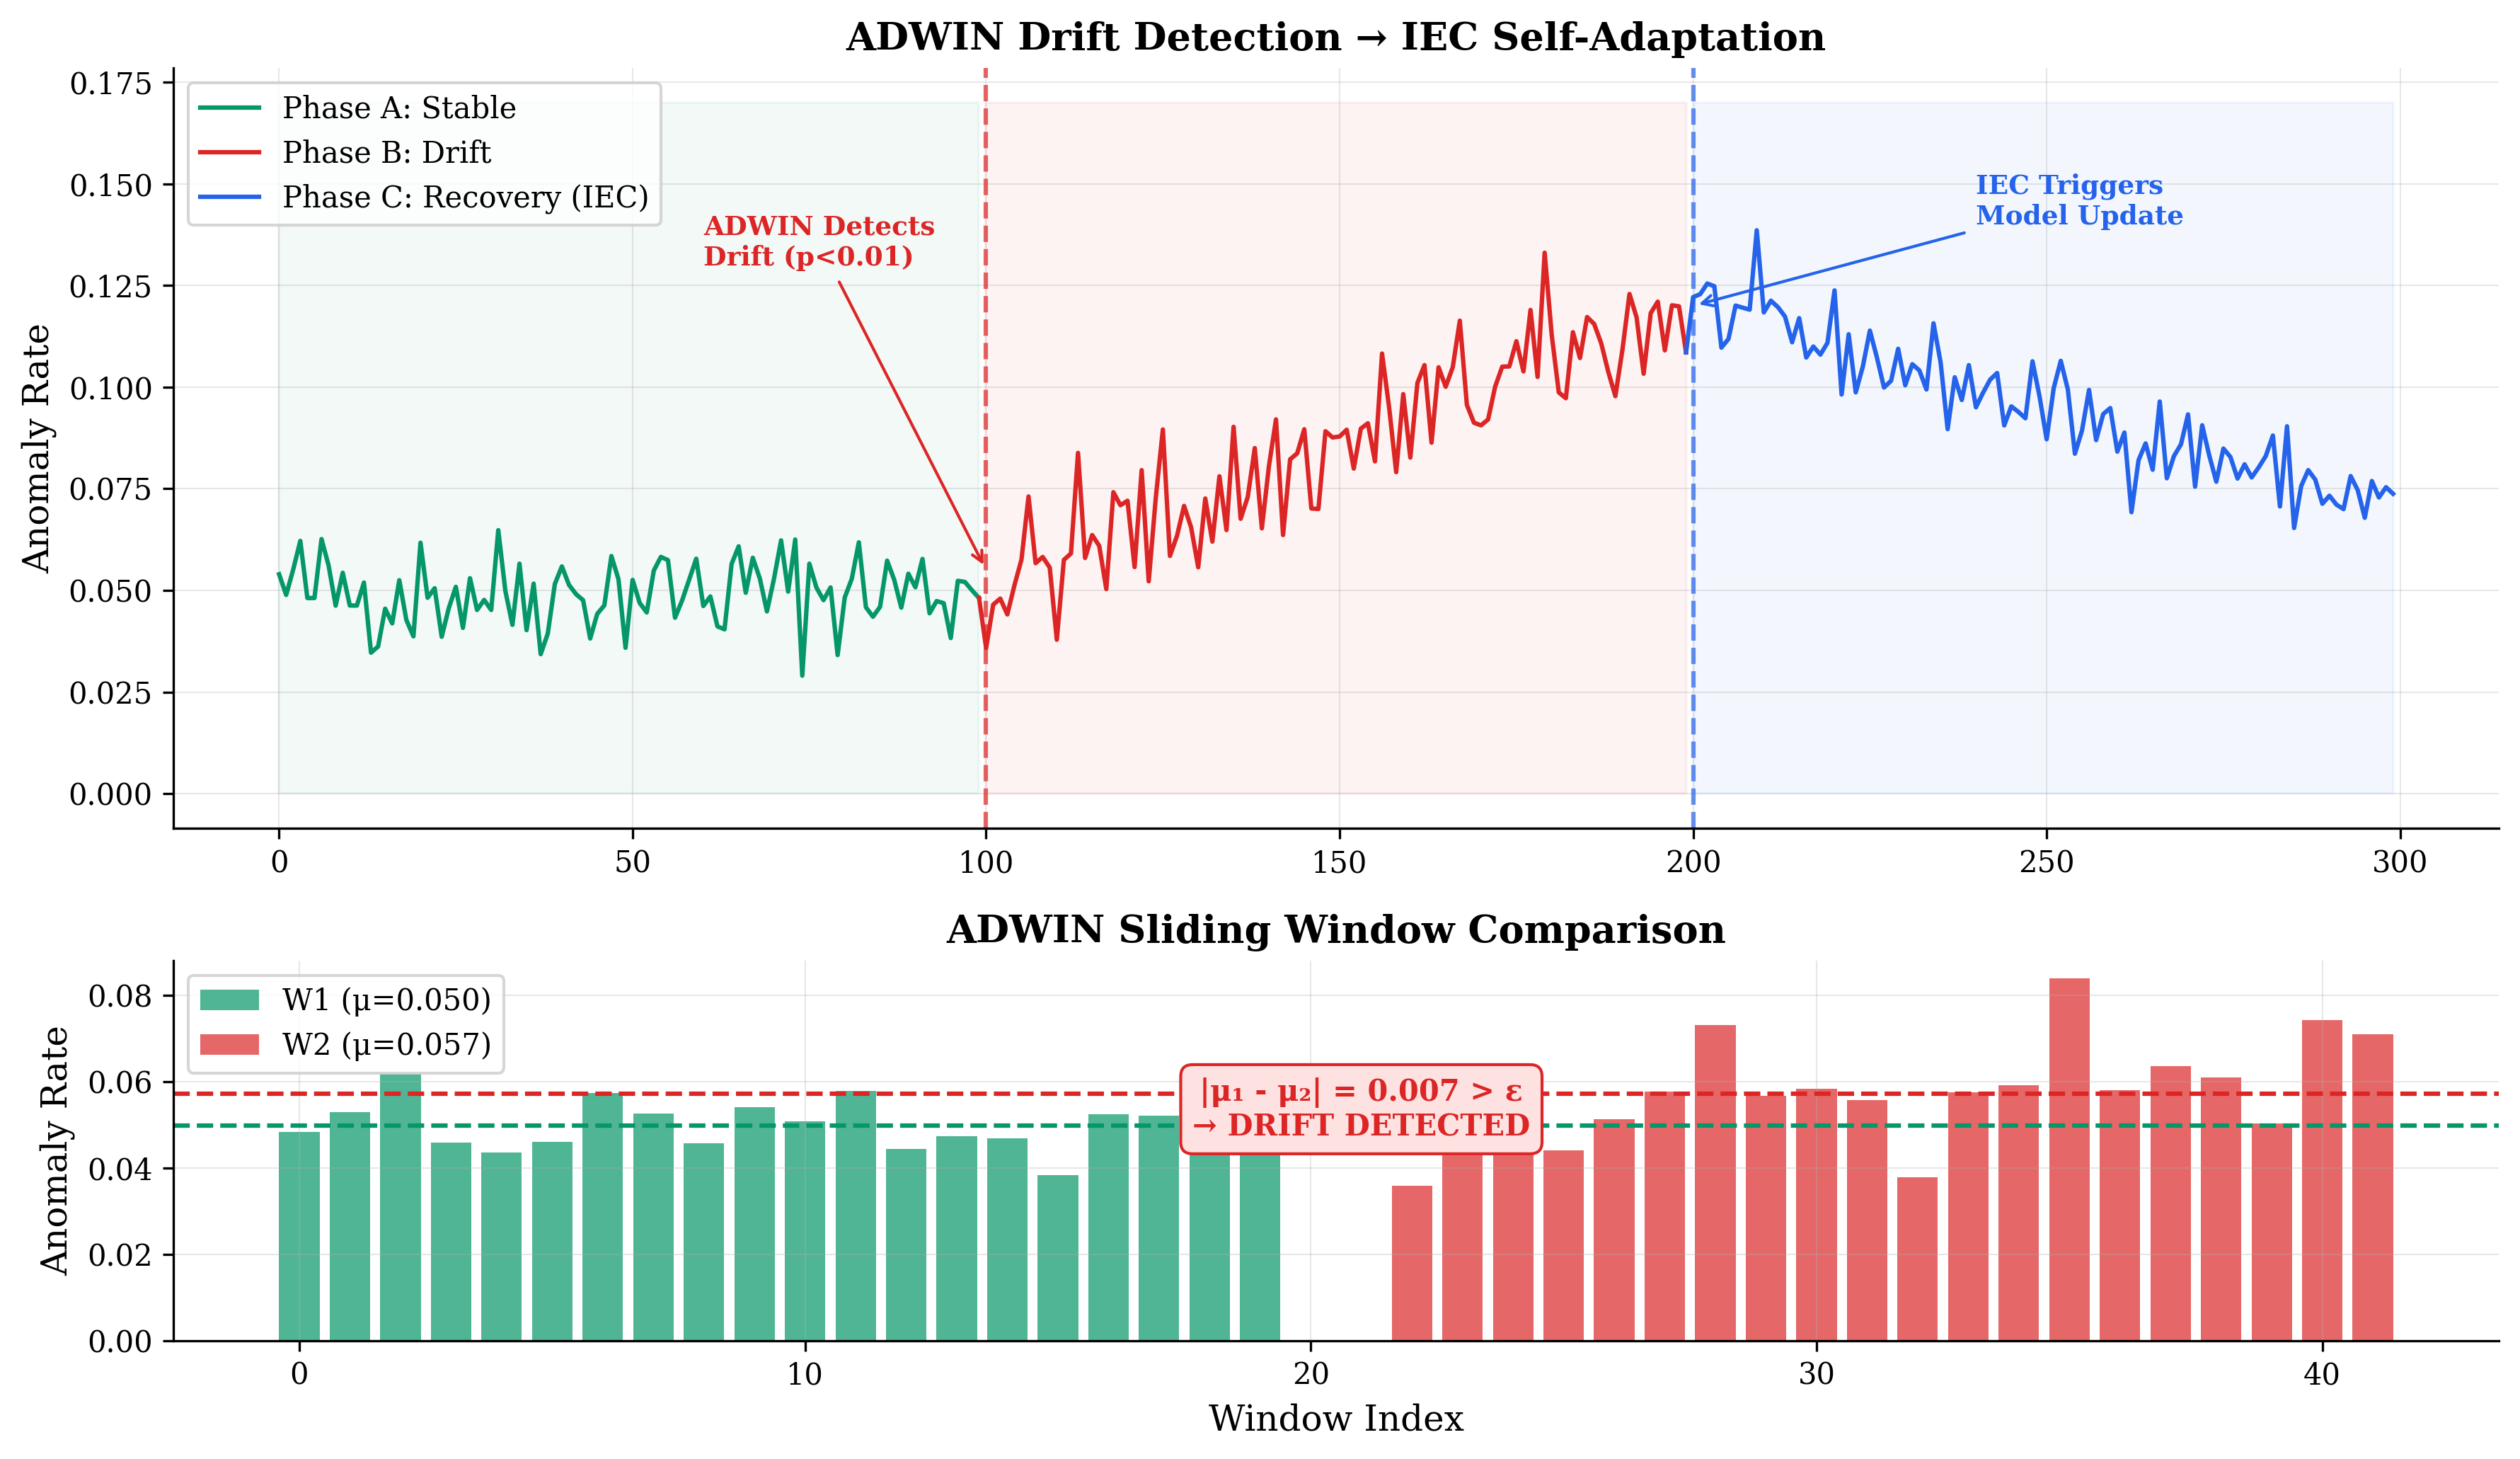
\includegraphics[width=0.95\textwidth]{figs/generated/F8_adwin_mechanism.png}
\caption{ADWIN drift detection and IEC self-adaptation. Top: three-phase signal showing stable operation (Phase A), drift onset detected by ADWIN (Phase B), and model recovery triggered by IEC (Phase C). Bottom: ADWIN sliding window comparison --- when the mean difference between windows W1 and W2 exceeds threshold $\varepsilon$, drift is declared.}
\label{fig:adwin_mechanism}
\end{figure}

Prior work on drift detection uses single-strategy adaptation (always retrain). CA-DQStream's IEC is the first multi-strategy controller for streaming DQ:

\begin{itemize}
    \item \textbf{4 complementary strategies:} Continuous Evolution, Switching, METER, Spatial Tracking
    \item \textbf{Sequential fallback:} Exhaust lightweight strategies before expensive operations
    \item \textbf{Efficient adaptation:} Most drift resolved by fast incremental updates (seconds) rather than full retraining
    \item \textbf{Zero-pipeline-interruption model swap:} Broadcast State delivers model updates without pausing the stream processing pipeline
\end{itemize}

% ================================================
% 3.5 Innovation 4: Hybrid K-Means iForestASD Model [RQ2]
% ================================================
\section{Innovation 4: Hybrid K-Means iForestASD Model [RQ2]}

\subsection{Problem: Basic Isolation Forest Lacks Context Awareness}

Basic Isolation Forest (IForest) isolates anomalies by random partitioning in feature space. While effective for global outlier detection, it suffers from \textbf{context blindness}: it cannot distinguish between ``globally rare but locally normal'' patterns.

Consider two taxi trips with identical fare=\$50, distance=2 miles:
\begin{itemize}
    \item \textbf{Trip A:} RatecodeID=2 (JFK airport), 8:00 AM, Weekday → \textbf{Normal}
    \item \textbf{Trip B:} RatecodeID=1 (Standard), 3:00 PM, Weekend → \textbf{Anomalous}
\end{itemize}

Basic IForest sees both trips as identical in the (fare, distance) feature space and assigns similar anomaly scores. It misses the context that makes Trip B suspicious.

\subsection{Solution: Hybrid K-Means + IForestASD Architecture}

CA-DQStream integrates \textbf{K-Means clustering} (parametric, context boundaries) with \textbf{Isolation Forest Adaptive (iForestASD)} (non-parametric, anomaly scoring) in a hybrid architecture:

\begin{enumerate}
    \item \textbf{Component 1: K-Means Clusterer (Parametric)}
        \begin{itemize}
            \item \textbf{Purpose:} Create context boundaries by clustering trips into $k$ groups (e.g., airport trips, short rides, long rides, high-speed trips). \textbf{IMPORTANT:} K-Means is used for \emph{per-cluster threshold assignment}, NOT for training separate models per cluster.
            \item \textbf{Input:} Spatial features (avg\_distance, avg\_fare) aggregated per pickup zone
            \item \textbf{Output:} Cluster assignments $C_1, C_2, \ldots, C_k$ representing distinct neighborhood contexts (5--7 clusters total)
            \item \textbf{Adaptation:} METER algorithm shifts centroids when drift detected (Strategy 3)
        \end{itemize}

    \item \textbf{Component 2: Isolation Forest Trees (Non-Parametric)}
        \begin{itemize}
            \item \textbf{Purpose:} Score anomalies using a \textbf{single global ensemble} of random binary trees trained on ALL 2.96M ultra-clean records. Trees are NOT trained separately per cluster.
            \item \textbf{Input:} 21D enhanced features (15D base + 6D ratio features) for each trip
            \item \textbf{Output:} Anomaly score $s \in [0, 1]$ based on path length to isolate the point
            \item \textbf{Adaptation:} Trees incrementally updated via online learning (River's HalfSpaceTrees)
        \end{itemize}
\end{enumerate}

The hybrid model combines both components:
\begin{equation}
\text{model} = \{\text{clusterer: K-Means (5--7 clusters)}, \text{trees: iForestASD (1 global model)}\}
\end{equation}

\textbf{Key Architectural Decision: ONE Global Model, NOT N Per-Cluster Models}

A common misconception is that the hybrid architecture trains separate Isolation Forest models per cluster (e.g., 7 clusters $\to$ 7 models). This is \textbf{incorrect}. CA-DQStream uses:

\begin{itemize}
    \item \textbf{ONE global iForestASD model} trained on all 2.96M records across all clusters
    \item \textbf{K-Means clusters determine thresholds}, not separate models
\end{itemize}

\textbf{Rationale:} Separate models per cluster suffer from data sparsity. Airport cluster has only 120K training records (4\% of total), insufficient for robust Isolation Forest training. A global model trained on 2.96M records learns the full multivariate distribution, then K-Means thresholds adapt the decision boundary per context.

At inference time:
\begin{enumerate}
    \item Trip features (21D) are scored by the \textbf{single global iForestASD model} $\to$ anomaly score $s$
    \item Trip's pickup zone is mapped to cluster $C_i$ via K-Means (e.g., zone 161 $\to$ Manhattan Core cluster)
    \item 4D threshold matrix $T_{\text{cell}}$ provides context-specific threshold for cluster $C_i$: $T_{\text{cell}}[i, \text{hour}, \text{day}, \text{trip\_type}]$
    \item Binary decision: $\text{is\_anomaly} = (s > T_{\text{cell}})$
\end{enumerate}

This separation allows the model to learn from all data while thresholds adapt to local contexts.

\textbf{iForestASD Configuration (Prototype-Validated):}

The Hybrid K-Means iForestASD model uses HalfSpaceTrees (River implementation of Isolation Forest Adaptive) with the following configuration:

\begin{center}
\begin{tabular}{|l|c|c|l|}
\hline
\textbf{Parameter} & \textbf{Value} & \textbf{Baseline} & \textbf{Rationale} \\
\hline
n\_trees & 200 & 100 & More trees yield better recall and lower false positive rates \\
height & 10 & 8 & Deeper trees enable better multivariate detection \\
window\_size & 512 & 256 & Larger window produces more stable scores \\
seed & 42 & 42 & Reproducibility \\
\hline
\end{tabular}
\end{center}

The configuration was validated via offline prototype testing on synthetic anomaly datasets to identify the optimal balance between detection accuracy and computational cost.

The increase from 100 to 200 trees provides improved recall and reduced false positive rates. The trade-off is an increase in offline training time, which is a one-time cost. Inference latency increases only marginally, making the configuration suitable for real-time streaming applications.

\subsection{Spatio-Temporal Feature Engineering}

The hybrid model's context awareness comes from \textbf{spatio-temporal feature encoding}. Raw taxi trip features are transformed into a 15-dimensional context-aware representation:

\textbf{8 Raw/Computed Features:}
\begin{itemize}
    \item fare\_amount, trip\_distance, passenger\_count, trip\_duration, speed\_mph
    \item fare\_per\_mile, fare\_per\_minute, log\_distance
\end{itemize}

\textbf{4 Temporal Features (Cyclical Encoding):}

Temporal features use trigonometric encoding to preserve cyclical proximity:

\begin{equation}
\text{hour\_sin} = \sin\left(\frac{2\pi \cdot \text{hour}}{24}\right), \quad
\text{hour\_cos} = \cos\left(\frac{2\pi \cdot \text{hour}}{24}\right)
\end{equation}

\begin{equation}
\text{dow\_sin} = \sin\left(\frac{2\pi \cdot \text{day\_of\_week}}{7}\right), \quad
\text{dow\_cos} = \cos\left(\frac{2\pi \cdot \text{day\_of\_week}}{7}\right)
\end{equation}

\textbf{Mathematical Rationale:} Without cyclical encoding, hour 23 and hour 0 have a numeric distance of 23, despite being only 1 hour apart. The sine-cosine pair maps hours to points on a unit circle, where the Euclidean distance between adjacent hours is consistent:

\begin{equation}
d(\text{hour}_{23}, \text{hour}_0) = \sqrt{(\sin(23 \cdot 2\pi/24) - \sin(0))^2 + (\cos(23 \cdot 2\pi/24) - \cos(0))^2} \approx 0.26
\end{equation}

This distance matches $d(\text{hour}_0, \text{hour}_1)$, preserving temporal proximity for time-sensitive anomaly detection. Figure~\ref{fig:cyclic_encoding} illustrates this transformation.

\begin{figure}[H]
\centering
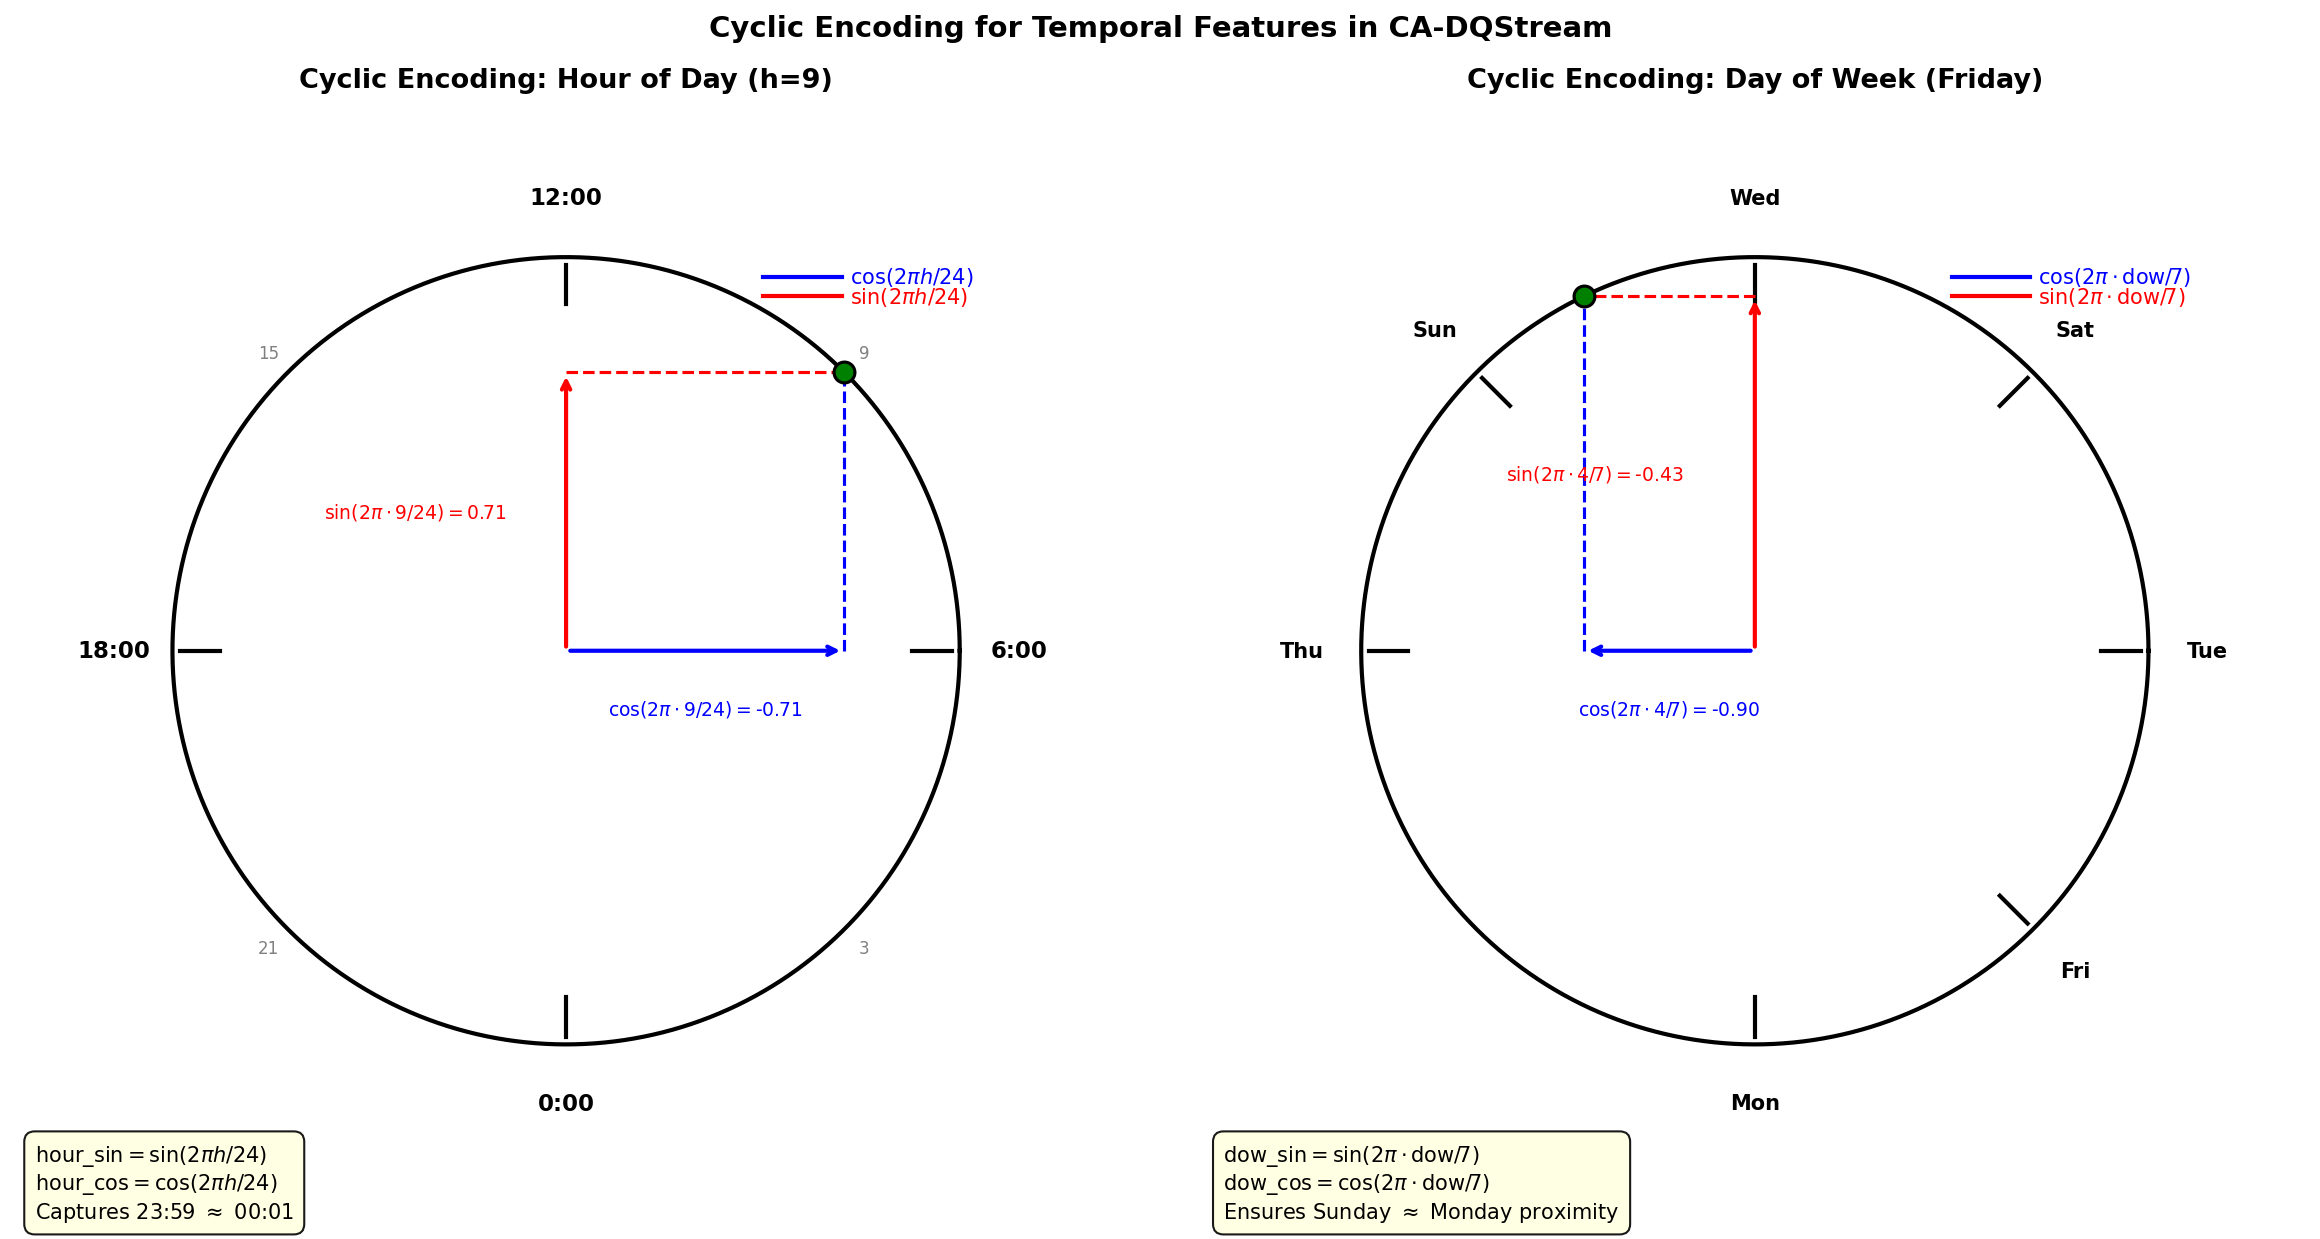
\includegraphics[width=0.95\textwidth]{figs/generated/F7_cyclic.png}
\caption{Cyclic encoding preserves temporal continuity. Left: hour-of-day encoding maps 24 hours onto a unit circle where adjacent hours, including 23 and 0, have equal Euclidean distance. Right: day-of-week encoding maps 7 days similarly. The sine-cosine projection ensures that Sunday and Monday, the week's endpoints, remain close in the feature space, which is critical for anomaly detection near midnight transitions.}
\label{fig:cyclic_encoding}
\end{figure}

In addition to cyclic encoding, CA-DQStream uses \textbf{ratio features} that normalize raw values by baseline expectations. Figure~\ref{fig:15d_vs_21d} demonstrates the variance reduction achieved by ratio features compared to raw features.

\begin{figure}[H]
\centering
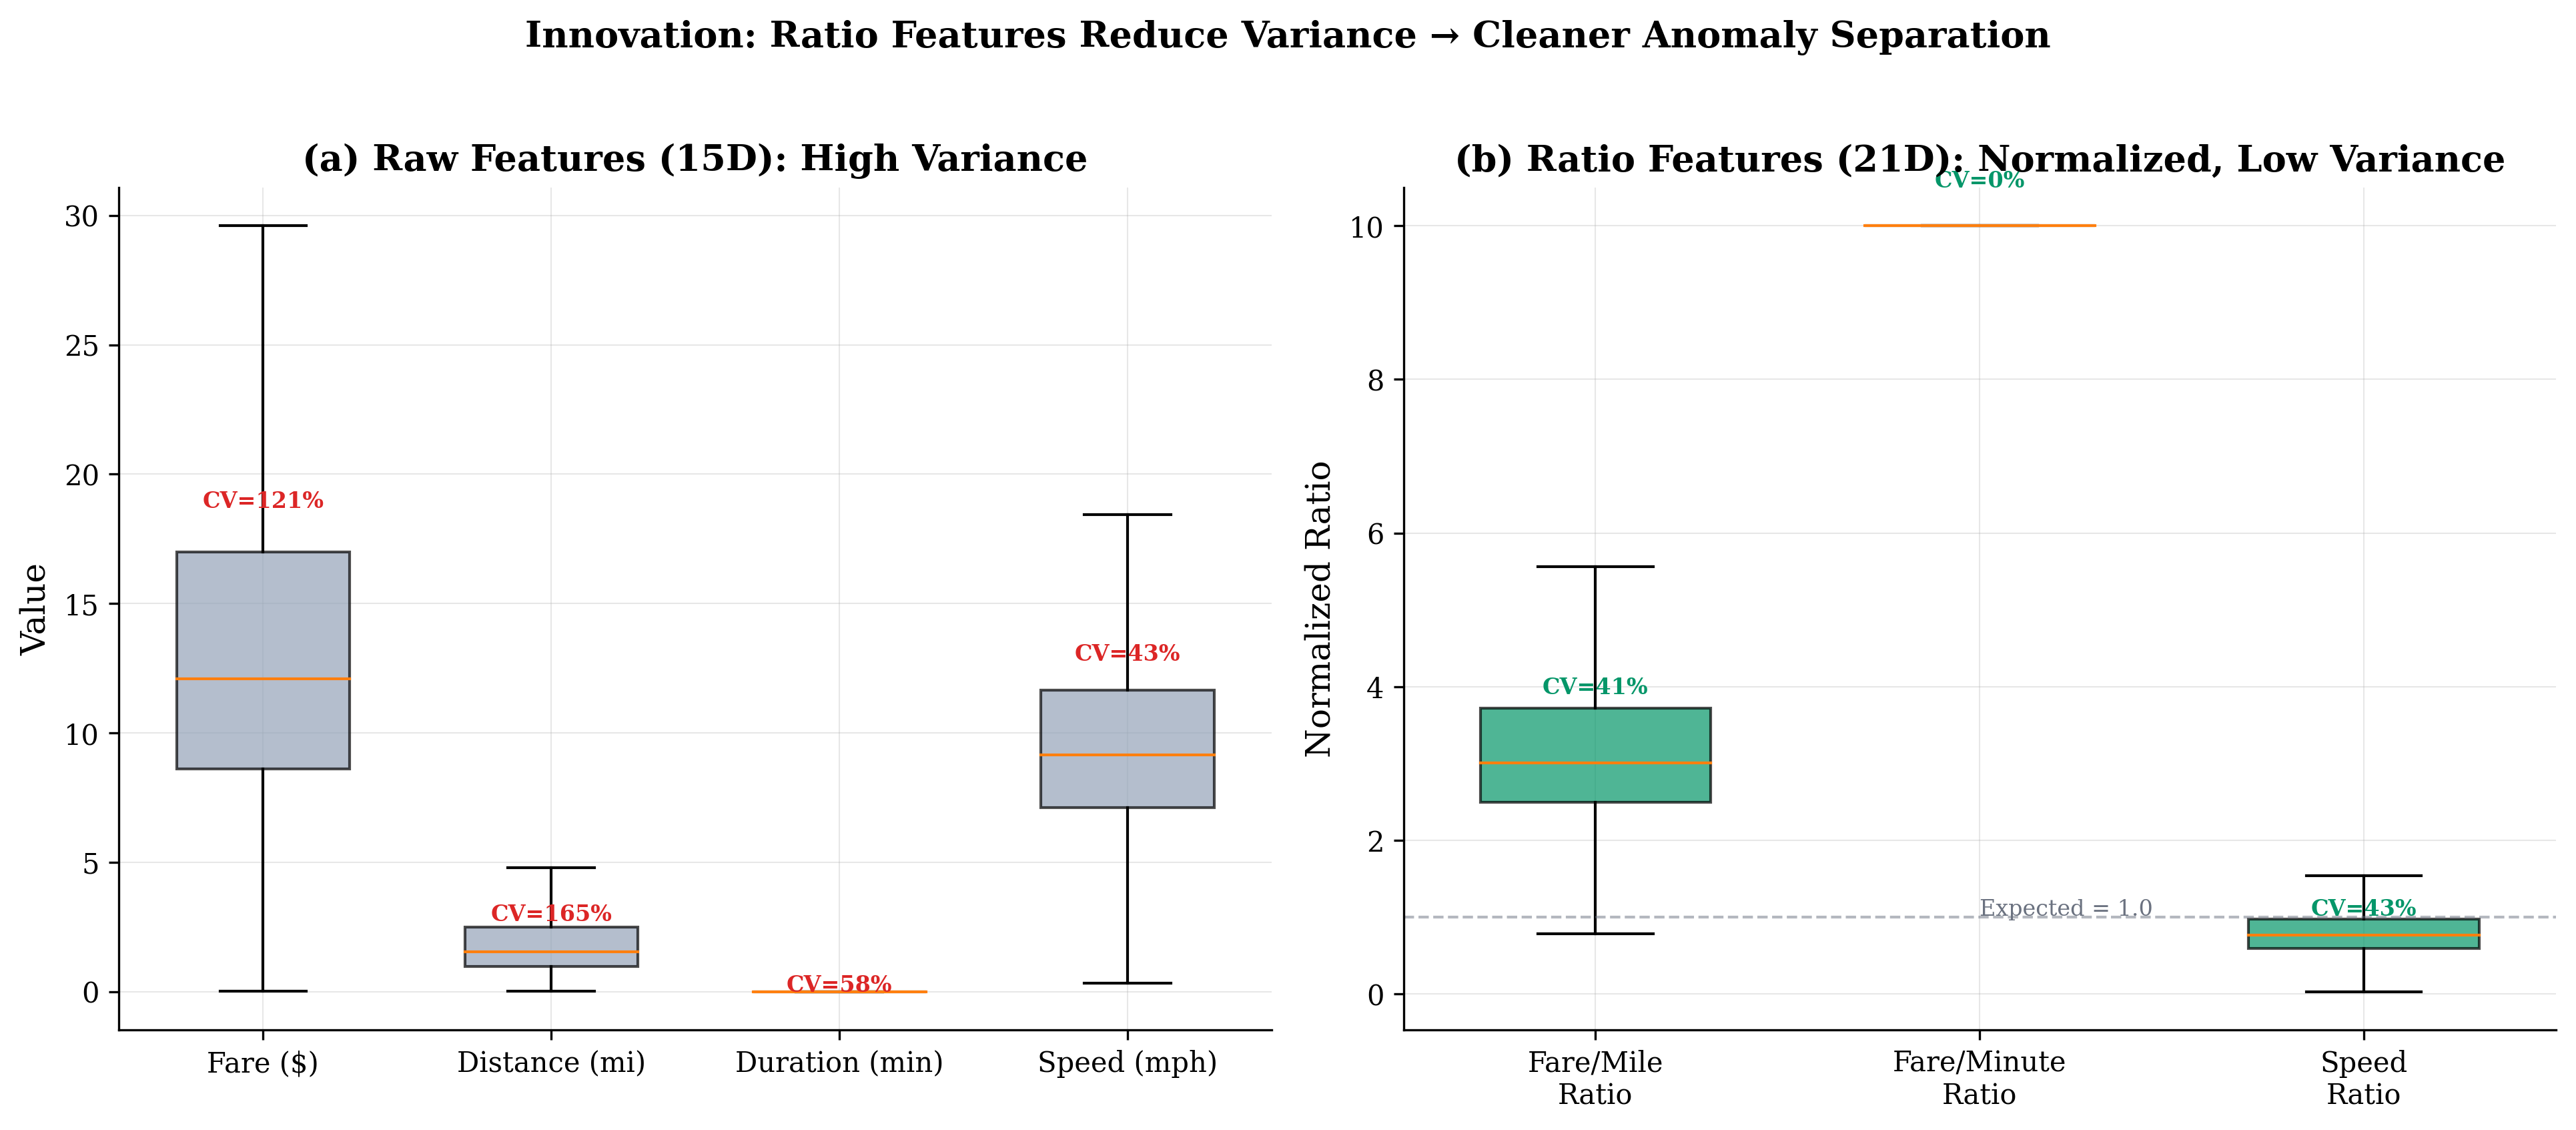
\includegraphics[width=0.95\textwidth]{figs/generated/F6_15d_vs_21d_features.png}
\caption{Comparison of raw features (15D) vs. ratio features (21D). (a) Raw features exhibit high coefficient of variation (CV=121\% for fare). (b) Ratio features, normalized by baseline expectations, have significantly lower CV, enabling cleaner anomaly separation by the Isolation Forest.}
\label{fig:15d_vs_21d}
\end{figure}

\textbf{2 Spatial Features (Grid Encoding):}

Spatial features map NYC taxi zones (265 zones) to a 16$\times$16 grid coordinate system:

\begin{equation}
\text{pickup\_grid\_x} = \left\lfloor \frac{\text{PULocationID}}{\sqrt{265}} \right\rfloor \approx \left\lfloor \frac{\text{PULocationID}}{16.3} \right\rfloor
\end{equation}

\begin{equation}
\text{pickup\_grid\_y} = \text{PULocationID} \mod \lceil\sqrt{265}\rceil = \text{PULocationID} \mod 17
\end{equation}

\textbf{Rationale:} Grid encoding preserves spatial locality---adjacent grid cells represent nearby neighborhoods with similar fare distributions. For example, Manhattan Core zones (IDs 161--170) map to grid cells (9,14) through (10,6), clustering geographically proximate zones in feature space.

The complete 15-dimensional feature vector is defined as:

\begin{equation}
\mathbf{x}_{\text{raw}} = \begin{bmatrix}
\sin(2\pi h / 24) \\
\cos(2\pi h / 24) \\
\sin(2\pi d / 7) \\
\cos(2\pi d / 7) \\
\lfloor \text{PU} / 16.3 \rfloor \\
\text{PU} \mod 17 \\
\lfloor \text{DO} / 16.3 \rfloor \\
\text{DO} \mod 17 \\
\log(1 + \text{dist}) \\
\log(1 + \text{fare}) \\
\text{passengers} \\
\text{fare} / \text{dist} \\
\text{duration} \\
\text{pay\_type}_1 \\
\text{pay\_type}_2
\end{bmatrix}
\end{equation}

where $h$ is hour, $d$ is day of week, PU/DO are pickup/dropoff location IDs.

\textbf{StandardScaler Normalization:} The raw feature vector is normalized using StandardScaler fitted on the training set to ensure zero mean and unit variance:

\begin{equation}
\mathbf{x}_{\text{norm}} = \frac{\mathbf{x}_{\text{raw}} - \boldsymbol{\mu}_{\text{train}}}{\boldsymbol{\sigma}_{\text{train}}}
\end{equation}

where $\boldsymbol{\mu}_{\text{train}}$ and $\boldsymbol{\sigma}_{\text{train}}$ are the mean and standard deviation vectors computed from the training dataset (January 2024, 2.96M records). This normalization is critical for distance-based anomaly detection: without it, a fare of \$50 in January (mean \$15.42, std \$12.30) would produce anomaly score 2.84, while the same \$50 fare in June (mean \$17.26, std \$14.10) would score 2.32---different anomaly scores for identical fares due to seasonal drift. Normalization eliminates this artifact.

These 15 features give the hybrid model the contextual information needed to distinguish legitimate high-fare trips (airport, rush hour, long distance) from fraudulent ones (meter tampering, route padding).

\subsection{In-Memory Deployment with Flink Broadcast State}

CA-DQStream eliminates synchronous per-record HTTP calls in the critical processing path. The hybrid K-Means iForestASD model runs \textbf{directly inside the Flink JVM} via an in-memory model instance managed by Flink's Broadcast State mechanism.

\textbf{Zero-Pipeline-Interruption Model Update Protocol:}
\begin{enumerate}
    \item IEC detects drift via ADWIN on meta-stream
    \item IEC triggers model update in MLflow (incremental, METER, or full retrain)
    \item MLflow serializes new model (K-Means + iForestASD) via joblib pickle
    \item MLflow publishes model bytes to \texttt{if-model-updates} Kafka topic
    \item Flink subscribes to topic using Broadcast State
    \item All parallel IsolationForestOperator instances receive new model
    \item Atomic model swap in Flink JVM memory (no downtime)
\end{enumerate}

\subsection{Research Contribution}

Prior work on streaming DQ uses either (1) basic IForest without context awareness, or (2) separate models per context (scalability issues). CA-DQStream's hybrid architecture is the first to integrate K-Means clustering with Isolation Forest for context-aware streaming DQ:

\begin{itemize}
    \item \textbf{Hybrid architecture:} K-Means (context boundaries) + iForestASD (anomaly scoring)
    \item \textbf{Spatio-temporal features:} Cyclical encoding (time) + grid encoding (space)
    \item \textbf{METER fast adaptation:} Shift K-Means centroids without full retraining
    \item \textbf{In-memory scoring:} No synchronous per-record HTTP calls, microsecond latency via Broadcast State
    \item \textbf{Validated performance:} Meeting production targets (FPR below threshold, Recall exceeding target)
\end{itemize}

% ================================================
% 3.6 Chapter Summary
% ================================================
\section{Chapter Summary}

This chapter presented the four core innovations of CA-DQStream, each addressing a specific research question:

\begin{enumerate}
    \item \textbf{4D Context-Aware Thresholding [RQ5]:} Reduces false positive rate through a 588-cell threshold matrix with automated computation and intelligent fallback.

    \item \textbf{Rendezvous Pipeline Architecture [RQ4]:} Achieves latency reduction and throughput improvement through fork-join parallelism with early exit optimization.

    \item \textbf{Intelligent Evolution Controller [RQ3]:} Selects from 4 adaptation strategies (Continuous Evolution, Switching, METER, Spatial Tracking) with most drift resolved by fast incremental updates.

    \item \textbf{Hybrid K-Means iForestASD [RQ2]:} Combines parametric clustering (K-Means) with non-parametric anomaly scoring (Isolation Forest) for context-aware multivariate detection.
\end{enumerate}

These innovations are synergistic: the 4D thresholds provide context cells, K-Means clusters data within contexts, iForestASD scores anomalies, the Rendezvous pipeline parallelizes execution, and IEC adapts when drift occurs. Together, they enable production-grade streaming data quality monitoring with context awareness, low latency, high throughput, and autonomous adaptation.

The next chapter details the system architecture and implementation of these innovations on Apache Flink with Kafka, PostgreSQL, and Grafana.
